\documentclass[tikz]{standalone}

\usepackage{circuitikz}

\begin{document}
	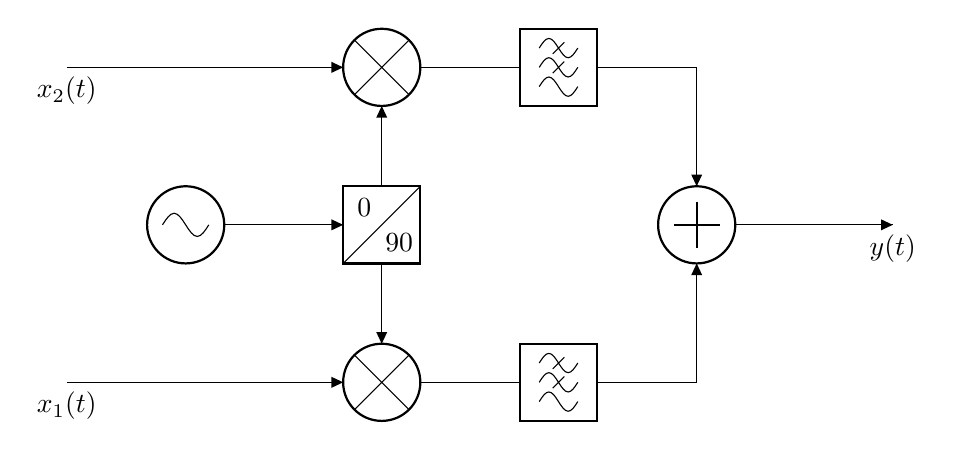
\begin{tikzpicture}
		\draw (0,0) node[below]{$x_1(t)$} (4,0)
            node[mixer](mixer){};
        \draw (0,0) to[short] (mixer.west) node[inputarrow, anchor=tip]{};
        \draw (2,2) node[oscillator](osc){} to[short] (mixer.west |- osc) node[inputarrow]{} node[twoportsplitshape, anchor=west, circuitikz/t1=0, circuitikz/t2=90](splitter){};
        \draw (splitter.south) to[short] (mixer.north) node[inputarrow, rotate=-90]{};
        \draw (0,4) node[below]{$x_2(t)$} to[short] (0,4-|mixer.west) node[inputarrow]{} node[mixer, anchor=west](mixer2){};
        \draw (splitter.north) to[short] (mixer2.south) node[inputarrow, rotate=90]{};
        \draw (splitter) ++(4,0) node[adder](adder){};
        \draw (mixer.east) to[lowpass] (mixer-|adder) to[short] (adder.south) node[inputarrow, rotate=90]{};
        \draw (mixer2.east) to[lowpass] (mixer2-|adder) to[short] (adder.north) node[inputarrow, rotate=-90]{};
        \draw (adder.east) to[short] ++(2,0) node[inputarrow]{} node[below]{$y(t)$};
	\end{tikzpicture}
\end{document}
